\chapter{PortAudio}\label{chap:lib}\label{app:portaudio}
As this project requires the usage of the sound card in a computer some interface is needed. A quick search on Google resulted in a countless number of possibilities for interfacing a C++ program with the sound card of a computer. The team decided on a set of requirements which the interface had to provide. Requirements are listed below:

\begin{itemize}
\item Easy-to-use application programming interface.
\item Cross platform.
\item Access to raw sample data.
\item Variable sample speed.
\item Support multiple streams.
\end{itemize}

The surface of several interfaces was scratched to see what they had to offer. Some of the possibilities are listed below:

\begin{description}
\item[RT Audio\footnote{}] was crap...
\footnotetext{\url{http://www.music.mcgill.ca/~gary/rtaudio/}}

\item[QT Multimedia\footnote{}] is developed by Nokia, and is a good suggestion as it comply with the requirements. The disadvantage is that core files from QT itself is needed which result in increased size of the developed software. Not that the size is specified as a requirement of the project itself but it also result in a superior complexity of the developed software itself, so QT Multimedia was discarded.
\footnotetext{\url{http://doc.qt.nokia.com/latest/qtmultimedia.html}}

\item[PortAudio\footnote{}] was finally chosen as the lowermost component of the software as it comply with the requirements mentioned above.  The reason for this final decision was based on the simplicity of the usage of PortAudio. Beside this point it is extremely adaptable which make it possible to use in a wide range of applications. A block diagram can be seen in figure \ref{fig:app_portaudio}.

\begin{figure}[!h]
	\begin{center}
	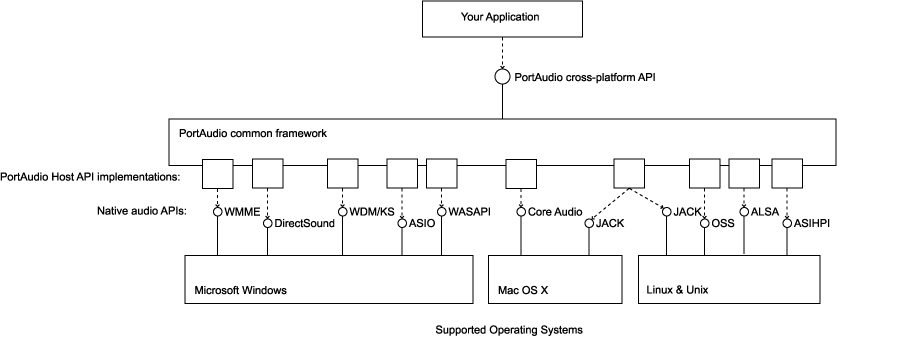
\includegraphics[scale=0.4,trim=0 0 0 0]{content/graphics/appendix/portaudio_architecture.png}%trim=l b r t
	\caption{This is an overview of the PortAudio interface.}
	\label{fig:app_portaudio}
	\end{center}
\end{figure}

\footnotetext{\url{http://www.portaudio.com/}}
\end{description}